\section{Metode}
\begin{figure}[H]
    \centering
    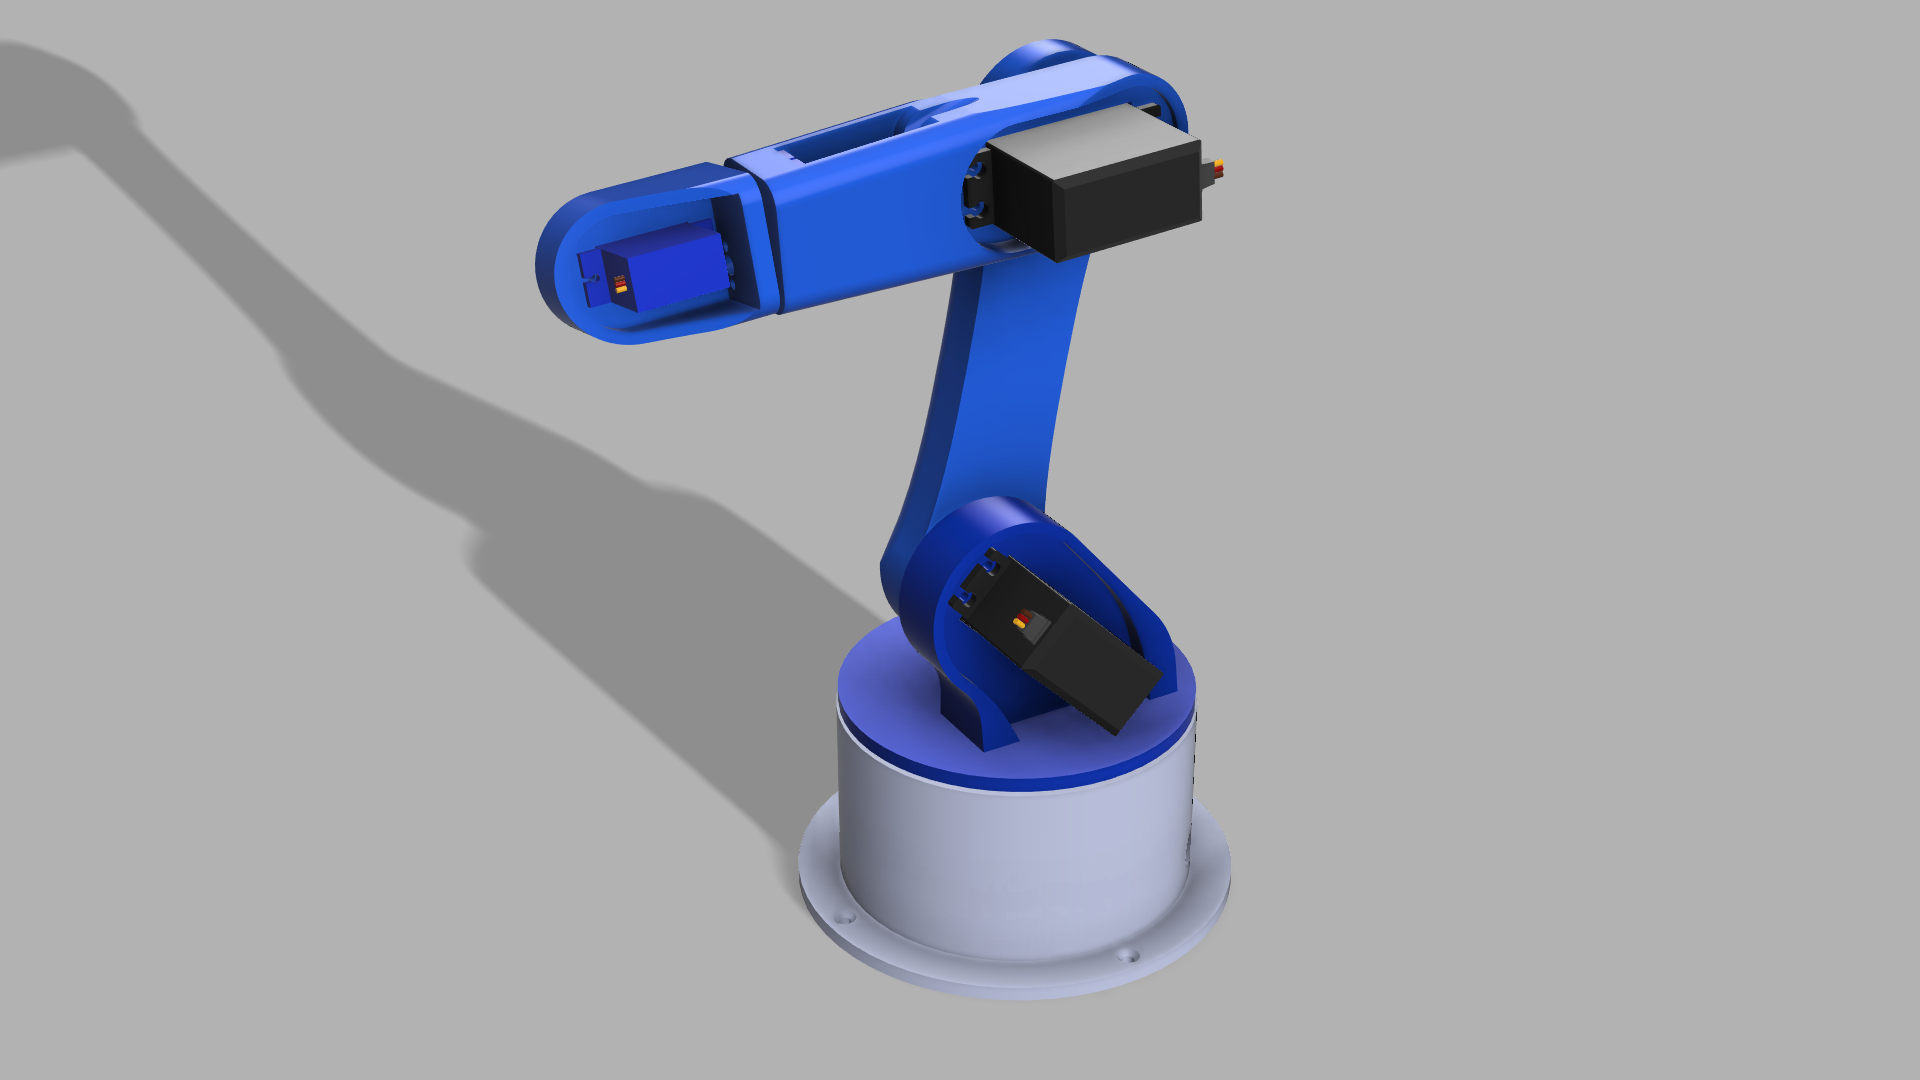
\includegraphics[width=0.5\linewidth]{Images/Arm_3D_Model.png}
    \caption{3D model av robot arm}
    \label{fig:3D_arm}
\end{figure}

\subsection{Testing før mottatt PCB}
Siden produksjon og levering av PCB-ene tok tid, var det viktig å verifisere at de sentrale komponentene og kommunikasjonsprotokollene fungerte før kortene kom i posten. Raspberry Pi-en ble stilt til rådighet av universitetet tidlig i prosjektet, og vi brukte derfor denne til å teste de ulike delene av systemet hver for seg på forhånd.

Først testet vi I2C-kommunikasjonen, ettersom denne er avgjørende for styringen av servomotorene. Ved hjelp av en frittstående PCA9685-modul koblet til Raspberry Pi-en kunne vi bekrefte at Pi-en oppdaget enheten på I2C-bussen, og at vi klarte å generere stabile PWM-signaler ut fra modulen. På denne måten fikk vi verifisert både selve I2C-oppsettet og at vi kunne styre en servomotor via PCA9685 før dette ble integrert på vårt eget kort.

\subsection{Kretsen}
Vi tok hva vi hadde i POR-en for å finne ut hvilke funksjoner som var nødvendige, og hvilke som kunne inkluderes om vi hadde plass til det. Vi fant ut at kortet skal gi ut fem PWM-signaler, tre knapper, muligheten strømtilførsel uten USB-C, fire ledige pins for I2C-kommunikasjon, samt tre HX711-brikker for loadcells.

\newcolumntype{P}[1]{>{\raggedright\arraybackslash}p{#1}}

\begin{center}
\footnotesize
\begin{longtable}{P{4.6cm} P{2.6cm} P{3.4cm} P{2.0cm} c}
\caption{Komponentliste (BOM) for PCB-ene.}\label{tab:bom}\\
\hline
\textbf{Description} & \textbf{Designator} & \textbf{Mfr. Part Number} & \textbf{Supplier} & \textbf{Qty} \\
\hline
\endfirsthead
\hline
\textbf{Description} & \textbf{Designator} & \textbf{Mfr. Part Number} & \textbf{Supplier} & \textbf{Qty} \\
\hline
\endhead
\hline
\endfoot
CAP ALUM 10UF 20\% 35V SMD & C1, C2, C5, C6, C7, C8 & EDK106M035A9BAA & Farnell & 6 \\
CAP CER 0.1UF 25V X7R 0603 & C3, C4, C9, C10, C11, C12 & C0603C104K3RAC7411 & Mouser & 6 \\
CAP CER 10UF 10V X5R 0603 & C13 & GRM188R61A106KE69D & Arrow & 1 \\
CC0603 100\,nF X7R 10\% 25\,V & C14, C15, C16, C17 & CC0603KPX7R8BB104 & Mouser & 4 \\
LED GREEN CLEAR CHIP SMD & D2, D3 & LTST-C193KGKT-5A & DigiKey & 2 \\
Female header, 40C, straight, 2.54\,mm, PBT/phos bronze & J2 & PPPC202LFBN-RC & DigiKey & 1 \\
CONN HEADER VERT 4POS 2.54MM & J3, J4, J5 & TSW-104-23-T-S & Arrow & 3 \\
CONN HEADER VERT 6POS 2.54MM & J6 & M20-9980346 & DigiKey & 1 \\
SQ post socket, TH, vertical, 2.54\,mm, 6-pin, female & J7 & SSW-103-01-L-D & DigiKey & 1 \\
0.025" SQ post header, TH, right-angle, 2.54\,mm, 2-pin, male & P5 & TSW-102-22-G-S-RA & Arrow & 1 \\
TRANS NPN 40V 0.2A SMD SOT23-3 & Q1, Q2, Q3, Q8, Q9 & MMBT3904-7-F & Farnell & 5 \\
Transistor PNP, 3-pin SC-75, Pb-free & Q5, Q6, Q7 & MMBT3906TT1G & Mouser & 3 \\
RES thick film, 20\,k$\Omega$, 1\%, 0.33\,W, 0603 & R1, R10, R13, R14, R17, R18 & CRCW060320K0FKEAHP & Arrow & 6 \\
RES thick film, 10\,k$\Omega$, 1\%, 0.2\,W, 0603, AEC-Q200 & R2, R4, R6, R7, R21 & SG73P1JTTD1002F & Mouser & 5 \\
RES thick film, 1\,k$\Omega$, 1\%, 0.1\,W, 0603, AEC-Q200 & R3, R5, R8, R9, R22 & RK73G1JTTD1001F & Farnell & 5 \\
RES SMD 100\,$\Omega$ 1\% 1/10W 0603 & R11, R12, R15, R16, R19, R20 & RT0603FRE07100RL & Arrow & 6 \\
RES thick film, 2.2\,k$\Omega$, 5\%, 0.1\,W, 0603 & R23 & RC1608J222CS & Arrow & 1 \\
RES thick film, 3.3\,k$\Omega$, 5\%, 0603 & R24 & CRGCQ0603J3K3 & Arrow & 1 \\
SWITCH TACTILE SPST-NO 0.05A 24V & SW1, SW2, SW3 & B3F-3122 & Arrow & 3 \\
\end{longtable}
\end{center}

Ved bruk av Raspberry Pi-en ble hovedprosesseringen og styringen forenklet. Pi-en ga en fornuftig måte å kommunisere med de andre komponentene på, via I2C, bit-banging og innlesing gjennom GPIO-pinnene.

Først fant vi ut hvordan PWM-utgangene skulle styres. PWM-signalet genereres ikke direkte av Raspberry Pi-en, men av en PCA9685 PWM-driver som Pi-en kommuniserer med over I2C. Figur \ref{fig:transistor} viser hvordan transistoren brukes. Signalet fra PCA chippen føres til PWM inngangen i kretsen, der strømmen går gjennom en motstand som begrenser basestrømmen til transistoren. Transistoren er en NPN BJT som opererer i en «common-emitter»-konfigurasjon, det vil si at emitteren er felles for inngangen og utgangen. Deretter er collector-pinnen koblet til en pull-up-motstand.

Når PWM-signalet er høyt, driver basestrømmen transistoren til saturation. Collectoren blir da trukket ned mot GND, og utgangen settes lav. Når PWM-signalet er lavt, går det ingen strøm til basen, og transistoren er «av». Da går det ingen strøm gjennom pull-up-motstanden, og utgangen trekkes høy til 5V.

\begin{figure}[H]
    \centering
    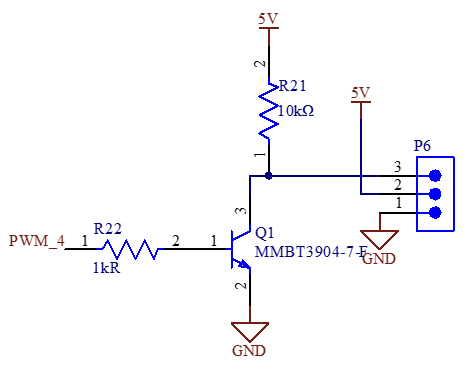
\includegraphics[width=0.5\linewidth]{Images/Transistor.png}
    \caption{Transistor oppsett}
    \label{fig:transistor}
\end{figure}



Hx711 kretsen var en ukjent komponent som krevet mye forskning. Hoved krets design/oppsett kom fra en produsent som leverer ferdig bygget Hx711 PCB-er. 

\subsection{Beste praksis for PCB-design}
\textbf{Avkoblingskondensatorer:} Hver aktive komponent ble utstyrt med avkoblingskondensatorer plassert så nær forsyningspinnene som mulig. PCA9685 og HX711-brikkene har dedikerte 100nF keramiske kondensatorer for å filtrere ut høyfrekvent støy, samt større 10 µF elektrolytt-/keramiske kondensatorer for å stabilisere forsyningsspenningen ved raske lastendringer. 

\textbf{Jordplan:} Kortet ble lagt ut med et sammenhengende jordplan (kobberfyll for GND). Et jordplan gir lav impedans tilbake til forsyningen og korte returbaner for signalstrømmene, noe som reduserer støy og gir mer stabile referansenivåer. Dette er særlig fordelaktig for de analoge målesignalene fra lastcellene, der et stabilt jordreferansenivå er avgjørende for nøyaktige avlesninger.

\textbf{Sporbredde for forsyning:} Spor som fører forsyningsstrøm (5V og 12V) ble tegnet merkbart bredere enn signalspor. Bredere spor har lavere resistans, noe som reduserer spenningsfallet og varmeutviklingen ved høyt strømtrekk. Dette er viktig i et system der servoer og pumpe kan trekke betydelig strøm samtidig.

\textbf{Separasjon av analoge signaler:} De analoge linjene fra lastcellene ble bevisst holdt adskilt fra PWM- og effektspor. Ved å unngå at følsomme målesignaler rutes parallelt med eller krysser støyende spor, reduseres innkobling av støy på HX711-avlesningene.



\subsection{Lodding}
    \hl{plassering av komponenter\\
    varmeovn\\
    through-hole deler}
\subsubsection{Enderinger}
    \hl{SDA pin\\
    floating ground\\
    pumpe int pin}

\subsection{Programmering}
\subsubsection{PCA9685}
PCA9685 chippen kommuniserer gjennom I2C, og siden PCA9685 er en ganske populær chip som blir brukt for å klare å styre flere servo motorer samtidig så eksisterte det allerede et bibliotek på python for denne chippen.

\subsubsection{HX711}
HX711 bruker sin egen type protokoll for kommunikasjon. Hvor RPi-en sender en 24 klokke pulser og for hver puls sender chippen ut et bit. Fra dette kan vi få data ut fra loadcellene som kan tolkes til vekt.

\subsection{main.py}
Programmet består av tre hoveddeler: import av nødvendige biblioteker, 
definisjon av matematiske funksjoner, og bygging av grafisk brukergrensesnitt (GUI).

\begin{figure}[H]
    \centering
    \includesvg[width=.75\linewidth]{Images/PackageDiagram.svg}
    \caption{Package Diagram}
    \label{fig:PackageDiagram}
\end{figure}

\subsubsection{Importerte biblioteker}
Følgende biblioteker blir importert:
\begin{itemize}
    \item \texttt{tkinter} — brukes til å lage det grafiske brukergrensesnittet (GUI)
    \item \texttt{time} — brukes til tidsmåling i PID-regulatoren
    \item \texttt{subprocess} — brukes til å starte eksterne prosesser, 
          som benchmark-programmet
    \item \texttt{math} — brukes til trigonometriske beregninger i invers kinematikk
    \item \texttt{ADAfruit} — 
    \item \texttt{hx711} — egen modul for avlesning av vektceller
\end{itemize}

\subsubsection{Tilstand}
Programmet bruker en global tilstandsmaskin med tre tilstander for fylleprosessen:
\begin{itemize}
    \item \texttt{idle} — systemet venter og overvåker vektcellene
    \item \texttt{moving} — armen beveger seg mot riktig glass
    \item \texttt{filling} — pumpen er aktiv og PID-regulatoren styrer fyllingen
\end{itemize}

\begin{figure}[H]
    \centering
    \includesvg[width=.75\linewidth]{Images/Tilstandsdiagram.svg}
    \caption{Tilstands Diagram}
    \label{fig:Tilstandsdiagram}
\end{figure}

\subsubsection{Invers kinematikk}
Funksjonen \texttt{solve\_ik()} beregner leddvinklene som kreves for å 
plassere endeffektoren i en gitt posisjon $(x, y, z)$ med ønsket 
orientasjon $\phi$.

\subsubsection{PID-regulator}
Funksjonen \texttt{pid\_control()} implementerer den diskrete PID-regulatoren. Regulatoren styrer pumpeeffekten 
basert på differansen mellom ønsket fyllingsnivå og målt vekt. 
Standardverdiene er satt til:
\begin{itemize}
    \item $K_p = 0.5$
    \item $K_i = 0.1$
    \item $K_d = 0.05$
\end{itemize}
Disse kan justeres direkte i GUI-et under kjøring.

\subsubsection{Fylleprosess}
Fylleprosessen styres av tre funksjoner:
\begin{itemize}
    \item \texttt{start\_fill()} — flytter armen til riktig glass og starter pumpen
    \item \texttt{begin\_pump()} — aktiverer pumpen og nullstiller PID-tilstanden
    \item \texttt{pid\_fill\_loop()} — kjører PID-regulatoren i en løkke med 
          \texttt{PID\_POLL\_MS} intervall (standard 200~ms) til målvekten er nådd
    \item \texttt{stop\_pump()} — slår av pumpen og returnerer til \texttt{idle}
\end{itemize}

Hvis vektcellen leser en negativ verdi under fylling tolkes dette som at 
glasset er løftet bort, og fyllingen avbrytes automatisk.

\subsubsection{Hovedløkke}
Funksjonen \texttt{main\_loop()} kjøres hvert 500~ms og overvåker alle 
tre vektcellene. Hvis systemet er aktivert og et glass er under 
terskelverdien \texttt{FILL\_THRESHOLD\_G} (standard 150~g), 
startes fylleprosessen automatisk for det aktuelle glasset.

\subsubsection{GUI}
GUI-et er bygget med \texttt{tkinter} og inneholder følgende seksjoner:
\begin{itemize}
    \item \textbf{Joint Control} — glidere for manuell styring av hvert ledd 
          (midje, skulder, albue, wrist) samt pumpe
    \item \textbf{Inverse Kinematics} — inntastingsfelt for målposisjon 
          $(x, y, z, \phi)$ og geometriparametere
    \item \textbf{Saved Positions} — lagring og avspilling av inntil 3 posisjoner med jevn interpolasjon
    \item \textbf{Load Cell} — sanntidsavlesning av alle tre vektceller med valg mellom live- og medianmodus
    \item \textbf{Tare og Kalibrering} — Kalibrering av innsamlet data fra loadcells og nullstillingsfunksjon
    \item \textbf{Fill Settings} — innstilling av terskel- og målvekt for fylling
    \item \textbf{Water Level} — fremdriftsindikatorer som viser fyllingsnivå 
          for hvert glass
    \item \textbf{PID Controller} — felt for $K_p$, $K_i$ og $K_d$ 
          med knapp for å anvende nye verdier under kjøring
\end{itemize}

\subsubsection{Avslutning}
Når programmet avsluttes frigjøres alle ressurser:
\begin{itemize}
    \item Vektcellene \texttt{sensor1}, \texttt{sensor2}, \texttt{sensor3} lukkes
    \item SPI-klokken \texttt{hx711.sck} lukkes
    \item Pumpe-GPIO-porten \texttt{pump\_fwd} lukkes
    \item I2C-bussen \texttt{i2c.bus} lukkes
\end{itemize}